\documentclass[tikz,border=2pt]{standalone}
\usepackage[T1]{fontenc}
\usepackage{amsmath}
\usetikzlibrary{arrows.meta,positioning,fit}
\begin{document}
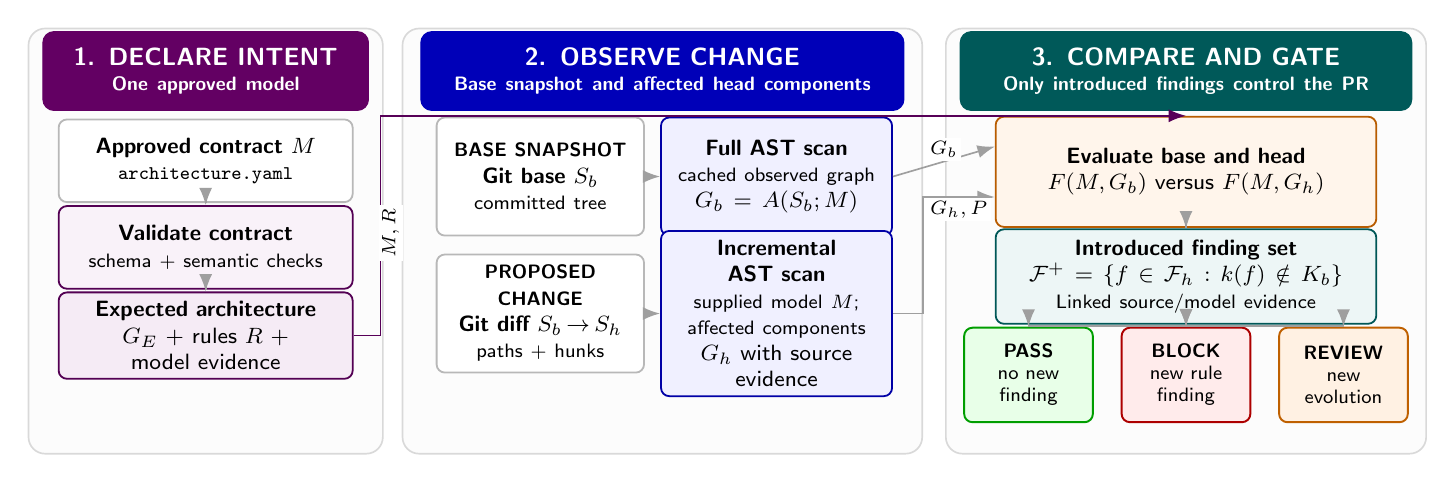
\begin{tikzpicture}[
    every node/.style={font=\sffamily\footnotesize},
    panel/.style={draw=gray!30, fill=gray!2, rounded corners=6pt, minimum height=54mm, line width=0.6pt},
    stage title/.style={text=white, rounded corners=4pt, align=center, minimum height=10mm, font=\sffamily\small\bfseries},
    declare title/.style={stage title, draw=violet!78!black, fill=violet!78!black, text width=39mm},
    observe title/.style={stage title, draw=blue!72!black, fill=blue!72!black, text width=59mm},
    gate title/.style={stage title, draw=teal!70!black, fill=teal!70!black, text width=55mm},
    card/.style={draw=gray!56, fill=white, rounded corners=3pt, align=center, minimum height=10.5mm, line width=0.65pt},
    input/.style={card, text width=35mm},
    process/.style={card, draw=violet!65!black, fill=violet!5, text width=35mm},
    artifact/.style={card, draw=violet!65!black, fill=violet!8, text width=35mm},
    lane input/.style={card, text width=24mm, minimum height=15mm},
    lane output/.style={card, draw=blue!65!black, fill=blue!6, text width=27mm, minimum height=15mm},
    compare/.style={card, draw=orange!72!black, fill=orange!8, text width=46mm, minimum height=14mm},
    finding/.style={card, draw=teal!68!black, fill=teal!7, text width=46mm, minimum height=12mm},
    decision/.style={rounded corners=3pt, align=center, minimum height=12mm, text width=14mm, font=\sffamily\scriptsize, line width=0.7pt},
    pass/.style={decision, draw=green!62!black, fill=green!9},
    block/.style={decision, draw=red!68!black, fill=red!8},
    review/.style={decision, draw=orange!75!black, fill=orange!11},
    flow/.style={-{Latex[length=2.2mm]}, semithick, draw=gray!75},
    intent flow/.style={-{Latex[length=2.2mm]}, semithick, draw=violet!68!black},
    edge label/.style={font=\sffamily\scriptsize, fill=white, inner sep=1.2pt, text=black}
  ]
    % Three stage cards keep authority, observation, and decision semantics separate.
    \node[panel, minimum width=45mm] (declarePanel) at (2.30,0) {};
    \node[panel, minimum width=66mm] (observePanel) at (8.10,0) {};
    \node[panel, minimum width=61mm] (gatePanel) at (14.75,0) {};

    \node[declare title] at (2.30,2.16) {1. DECLARE INTENT\\[-0.7mm]{\scriptsize One approved model}};
    \node[observe title] at (8.10,2.16) {2. OBSERVE CHANGE\\[-0.7mm]{\scriptsize Base snapshot and affected head components}};
    \node[gate title] at (14.75,2.16) {3. COMPARE AND GATE\\[-0.7mm]{\scriptsize Only introduced findings control the PR}};

    \node[input] (model) at (2.30,1.02) {\textbf{Approved contract $M$}\\{\scriptsize\texttt{architecture.yaml}}};
    \node[process] (validate) at (2.30,-0.08) {\textbf{Validate contract}\\{\scriptsize schema + semantic checks}};
    \node[artifact] (intent) at (2.30,-1.20) {\textbf{Expected architecture}\\$G_E$ + rules $R$ + model evidence};

    \node[lane input] (base) at (6.55,0.82) {{\scriptsize\bfseries BASE SNAPSHOT}\\\textbf{Git base $S_b$}\\{\scriptsize committed tree}};
    \node[lane output] (baseGraph) at (9.55,0.82) {\textbf{Full AST scan}\\{\scriptsize cached observed graph}\\$G_b=A(S_b;M)$};
    \node[lane input] (head) at (6.55,-0.92) {{\scriptsize\bfseries PROPOSED CHANGE}\\\textbf{Git diff $S_b\!\to\!S_h$}\\{\scriptsize paths + hunks}};
    \node[lane output] (headGraph) at (9.55,-0.92) {\textbf{Incremental AST scan}\\{\scriptsize supplied model $M$; affected components}\\$G_h$ with source evidence};

    \node[compare] (conformance) at (14.75,0.88) {\textbf{Evaluate base and head}\\$F(M,G_b)$ versus $F(M,G_h)$};
    \node[finding] (findingDelta) at (14.75,-0.45) {\textbf{Introduced finding set}\\$\mathcal{F}^{+}=\{f\in\mathcal{F}_h:k(f)\notin K_b\}$\\{\scriptsize Linked source/model evidence}};
    \node[pass] (passDecision) at (12.75,-1.70) {\textbf{PASS}\\no new finding};
    \node[block] (blockDecision) at (14.75,-1.70) {\textbf{BLOCK}\\new rule finding};
    \node[review] (reviewDecision) at (16.75,-1.70) {\textbf{REVIEW}\\new evolution};

    \draw[flow] (model) -- (validate);
    \draw[flow] (validate) -- (intent);
    \draw[flow] (base) -- (baseGraph);
    \draw[flow] (head) -- (headGraph);

    \draw[intent flow] (intent.east) -- ++(0.34,0) |- (conformance.north);
    \node[edge label, rotate=90] at (4.65,0.10) {$M,R$};
    \draw[flow] (baseGraph.east) -- node[edge label, above] {$G_b$} ([yshift=3.2mm]conformance.west);
    \draw[flow] (headGraph.east) -- ++(0.38,0) |- node[edge label, near end, below] {$G_h,P$} ([yshift=-3.2mm]conformance.west);
    \draw[flow] (conformance) -- (findingDelta);

    \coordinate (decisionHub) at (14.75,-1.08);
    \draw[flow] (findingDelta.south) -- (decisionHub);
    \draw[flow] (decisionHub) -| (passDecision.north);
    \draw[flow] (decisionHub) -- (blockDecision.north);
    \draw[flow] (decisionHub) -| (reviewDecision.north);
  \end{tikzpicture}
\end{document}
